\section{Complessità di tempo}
\subsection{Misure di Complessità}
Comsideriamo il linguaggio $A=\{0^k1^k\mid k \geq 0\}$
\begin{itemize}
  \item Che tipo di linguaggio è?
  \item È \g{decidibile}?
  \item Quanto \g{tempo} serve ad una TM a nastro singolo per decidere questo 
    linguaggio?
\end{itemize}
\paragraph{Definizione}
\begin{itemize}
  \item Sia $M$ una TM \g{deterministica} che si \g{ferma} su tutti gli input
  \item Il \g{tempo di eseguzione} (o \g{complessità di tempo}) di $M$ è
    la funzione $f:\mathbb{N} \mapsto\mathbb{N}$ tale che $f(n)$ è 
    il numero massimo di passi che $M$ utilizza su un input di lunghezza $n$.
  \item Se $f(n)$ è il tempo di esecuzione di $M$, diciamo che $M$ è una TM
    \g{di tempo $f(n)$}
  \item Useremo $n$ per rappresentare la \g{lunghezza dell'input}
  \item Ci interesseremo dell'\g{analisi del caso pessimo}
\end{itemize}
\subsection{Notazione $O$-grande}
\begin{itemize}
  \item \g{Analisi asintotica}: valuta il tempo di esecuzione su input grandi 
  \item Considera solo il \g{termine di ordine maggiore} e \g{ignora i coefficienti}
    \begin{definition}
      Date due funzioni $f,g$, diciamo che $f(n) = O(g(n))$ se esistono interi positivi
      $c, n_0$ tali che per ogni $n\geq n_0$
      \begin{displaymath}
        f(n)\leq c g(n)
      \end{displaymath}
      $g(n)$ è un \g{limite superiore asintotico} per $f(n)$ 
    \end{definition}
\end{itemize}
\subsection{Analisi di complessità}
Analizziamo questa TM per $A=\{0^k1^k\mid g\geq 0\}$\\
$M_1 =$ ``Su input $w$:
\begin{enumerate}
  \item Scorrere il nastro e \textit{rifiuta} se trova uno 0 a destra di un 1
  \item Ripete finché il nastro contiene almeno uno 0 e un 1
  \item Scorre il nastro cancellando uno 0 e un 1
  \item Se rimane almeno uno 0 dopo che ogni 1 è stato cancellato, 
    o se rimane almeno un 1 dopo che ogni 0 è stato cancellato, \textit{rifiuta}. 
    Altrimenti, se non rimangono né 0 né 1 sul nastro, \g{accetta}''
\end{enumerate}
\subsection{Classi di complessità di tempo}
\begin{definition}
  Sia $t:\mathbb{N}\mapsto\mathbb{N}$ una funzione\\
  La \g{classe di complessità di tempo $TIME(T(N))$} è l'insieme di tutti i 
  linguaggi che sono \g{decisi} da una \g{TM in tempo $O(t(n))$}
  \begin{itemize}
    \item Questo è diverso dalle classi di linguaggi discusse in precedenza, 
      che si concentravano sulla \g{computabilità}
    \item Questa classificazione si concentra sul \g{tempo necessario}
      per decidere il linguaggio.
  \end{itemize}
\end{definition}
\paragraph{Possiamo fare di meglio?} Dall'analisi che abbiamo fatto, sappiamo che 
$$ A=\{0^k1^k\mid k\geq 0\}$$
appartiene alla classi di complessità di tempo \g{$TIME(n^2$}, perché $M_1$ 
decide $A$ in tempo $O(n^2)$
\paragraph{MA} Esiste una macchina che decide $A$ in modo \g{asintoticamente più veloce}?
\paragraph{Miglioriamo $M_1$}\g{Idea}: cancelliamo metà degli 0 e metà degli 1 ad
ogni scansione
$M_2=$ ``Su input $W$:
\begin{enumerate}
  \item Scorre il nastro e \g{rifiuta} se trova uno 0 a destra di un 1
  \item Ripete finché il nastro contiene almeno uno 0 ed un 1
  \item Scorre il nastro e controlla se il numero totale di 0 e 1 rimasti
    è pari o dispari. Se è dispari, \textit{rifiuta}
  \item Scorre il nastro, cancellando prima ogni secondo 0 a partire dal primo
    0, poi cancellando ogni secondi 1 a partire dal primo 1.
  \item se nessuno 0 e nessun 1 rimangono sul nastro \g{acetta}. 
    Altrimenti \textit{rifiuta}
\end{enumerate}
\paragraph{Possiamo fare ancora meglio?}
\begin{itemize}
  \item Possiamo trovare una TM che decide $A$ in $O(n)$?
  \item \g{Problema}: non esiste una TM \g{a nastro singolo} che è in grado di decidere 
    $A$ in tempo $O(n)$.
  \item Possiamo farlo se la TM \g{ha un secondo nastro}
  \item \g{Importante}: la complessità di tempo dipende dal \g{modello di calcolo}
  \item La \g{Tesi di Church-Turing} implica che tutti i modelli di calcolo ``ragionevoli''
    siano equivalenti.
  \item \g{in pratica}: discuteremo qunto questa differenza sia importante (o meno) 
    per il nostro sistema di classificazione più avanti. 
\end{itemize}
\g{Idea}: usiamo il secondo nastro per contare 0 e 1
$M_2 =$ ``Su input $w$:
\begin{itemize}
  \item Scorre il nastro 1 e \textit{rifiuta} se trova uno 0 a destra di un 1
  \item Scorre i simboli 0 sul nastro 1 fino al primo 1. 
    Contemporaneamente, copia ogni 0 sul nastro 2.
  \item Scorre i simboli 1 sul nastro 1 fino alla fine dell'input. 
    Per ogni 1 letto sul nastro 1, cancella uno 0 sul nastro 2.
    Se ogni 0 è stato cancellato prima di aver letto tutti gli 1, \textit{rifiuta}
  \item Se tutti gli 0 sono stati cancellati, \g{accetta}. 
    Se rimane qualche 0, \textit{rifiuta}
\end{itemize}
\subsection{Relazione di complessità tra modelli}
\subsubsection{Singolo nastro vs. Multinastro}
\begin{theorem}
  Sia $t(n)$ una funzione tale che $t(n) \leq n$. Ogni TM \g{multinastro}
  di tempo $t(n)$ ammette una TM equivalente a \g{nastro singolo} di tempo 
  $O(t^2(n))$.
\end{theorem}
\begin{itemize}
  \item Ricordiamo la dimostrazione di come convertire una TM da multinastro 
    a nastro singolo.
    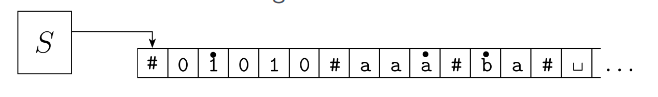
\includegraphics[scale=0.5]{img/nastro.png}
  \item Dobbiamo determinare quanto tempo ci vuole per simulare ogni passo 
    della macchina multinastro sulla TM a nastro singolo. 
\end{itemize}
\subsubsection{TM non deterministiche}
\begin{theorem}
  Sia $N$ una TM non deterministica che è anche un \g{decisore}. 
  Il \g{tempo di esecuzione} di $N$ è la funzione $f: \mathbb{N}\mapsto \mathbb{N}$
  tale che $f(n)$ è il massimo numero di passi che $N$ usa per ognuno dei rami di computazione, 
  su input di lunghezza $n$. 
\end{theorem}
\paragraph{Nota Bene} la definizione di tempo di esecuzione per le TM non deterministiche 
non è destinato a corrispondere ad un qualche dispositivo di calcolo reale. 
È uno strumento teorico che utilizziamo per comprendere i problemi computazionali.\\
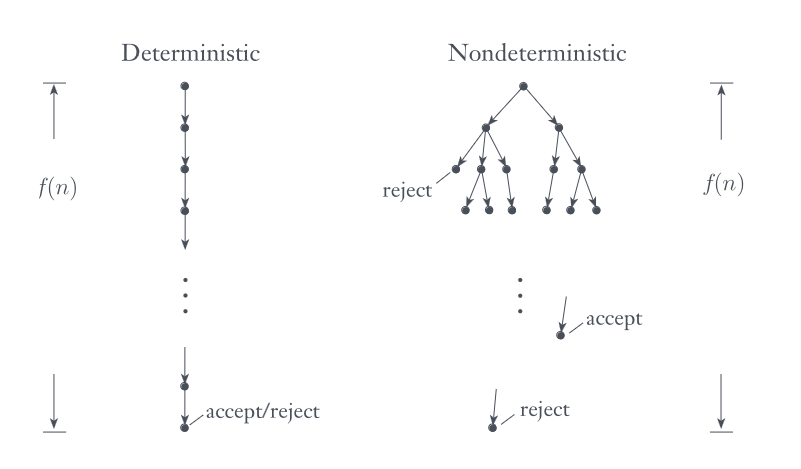
\includegraphics[scale=0.5]{img/tm_non_deterministiche.png}
\subsubsection{Determinismo vs. Non determinismo}
\begin{theorem}
  Sia $t(n)$ una funzione tale che $t(n)\leq n$. Ogni TM \g{non deterministica}
  di tempo $t(n)$ ammette una TM equivalente a \g{nastro singolo} di tempo 
  $2^{O(t(n))}$.
\end{theorem}
\paragraph{Dimostrazione}
\begin{itemize}
  \item Sia $N$ una TM non deterministica di tempo $t(n)$ 
  \item Costruiamo una TM deterministica $D$ che simula $N$. 
  \item $D$ è una TM \g{multinastro}. Qual è la complessità quando viene 
    convertita in una TM a nastro singolo? 
\end{itemize}
